% Load per-case macros and prerequisites
% Shared macros for per‑case reports
\newcommand{\CaseID}{tubbs\_fire}
\newcommand{\CaseTitle}{2017 Tubbs Fire Reconstruction}
\newcommand{\CaseOwner}{Yiren Qin}
\newcommand{\CaseVersion}{v0.1}
\newcommand{\CaseDate}{\today}
% Auto-generated metrics_macros.tex
\makeatletter
\newcommand{\DefineMetric}[2]{\expandafter\def\csname metric@#1\endcsname{#2}}
\newcommand{\Metric}[1]{%
  \ifcsname metric@#1\endcsname
    \csname metric@#1\endcsname
  \else
    \textbf{??}%
  \fi}
\newcommand{\MetricOr}[2]{%
  \ifcsname metric@#1\endcsname
    \csname metric@#1\endcsname
  \else
    #2%
  \fi}
\newcommand{\IfMetricTF}[3]{%
  \ifcsname metric@#1\endcsname
    #2%
  \else
    #3%
  \fi}
\makeatother

\DefineMetric{error_hrr_mean_rel}{0.000314}
\DefineMetric{error_dfc_mean_rel}{1.8e-05}
\DefineMetric{error_rad_mean_rel}{0.000288}

\documentclass[../report/case_report.tex]{subfiles}
\begin{document}

\subsection*{Case Summary}
\textbf{Case ID:} \CaseID\\
\textbf{Objective:} Validate Tubbs fire spreading against VIIRS observation


\subsection{Assumptions}
List assumptions concisely:
\begin{itemize}[nosep]
\item Homogeneous fuel; no spotting; steady uniform wind.
\item 2D structured grid, constant \(\Delta x = \Delta y\).
\item Boundary conditions: specify.
\end{itemize}


\subsection{Simulation Setup}
Key parameters and configuration choices (in elmfire.data.in). Cite the specific ELMFIRE config and any pre/post processing steps.


\subsubsection{Input Data}
Describe input rasters, constants, initial conditions.


\subsubsection{Numerical Controls}
Mesh resolution, Time step(CFL), level-set solver options, etc.


\subsection{Expected Results and Reasoning}
Derive the expected behavior (analytical solution or literature correlations). Include equations and parameter substitutions.


\subsection{Acceptance Criteria}
Define quantitative pass/fail criteria (e.g., RMSE\,\(\leq\)\,\SI{5}{\percent}).


\subsection{Results}
\begin{table}[h]
  \centering
  \begin{tabular}{l r r r}
    \toprule
    Metric & Value & $t_{simu}$ & $t_{observ}$\\ 
    \midrule
    $\kappa$(5.5 hr) & \Metric{kappa_1} & \Metric{t_simu_1} & \Metric{t_viirs_1} \\
    $\kappa$(12.0 hr) & \Metric{kappa_2} & \Metric{t_simu_2} & \Metric{t_viirs_2} \\
    \bottomrule
  \end{tabular}
  \caption{Cohen's Kappa values for available frames.}
  \label{tab:cohen_kappa}
\end{table}

\begin{figure}[h]
  \centering
  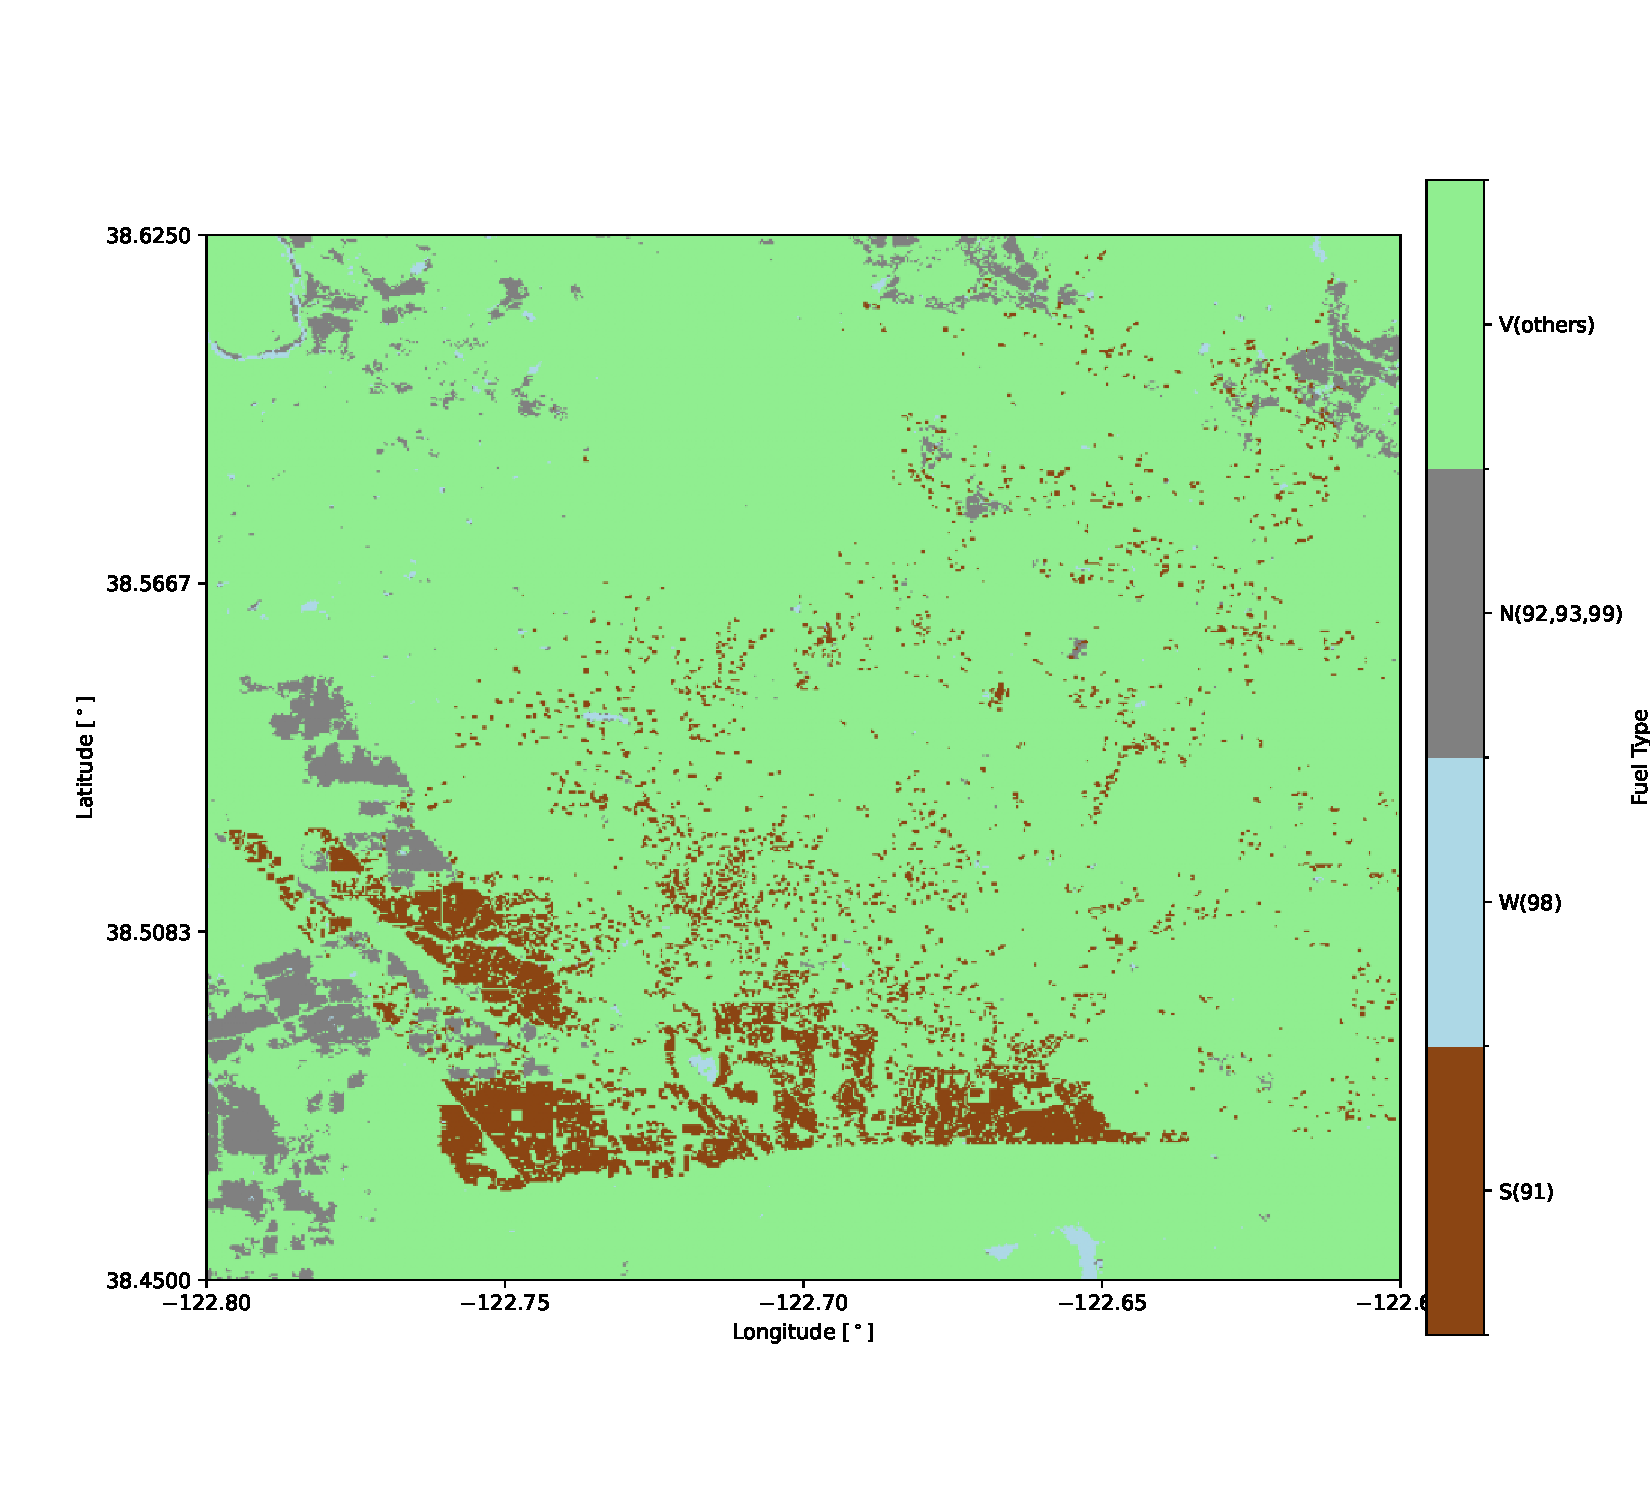
\includegraphics[width=0.7\textwidth]{../figures/fuelmap_categorical.pdf}
  \caption{Categorical fuel map used in the simulation domain.}
  \label{fig:fuelmap_categorical}
\end{figure}

\begin{figure}[h]
  \centering
  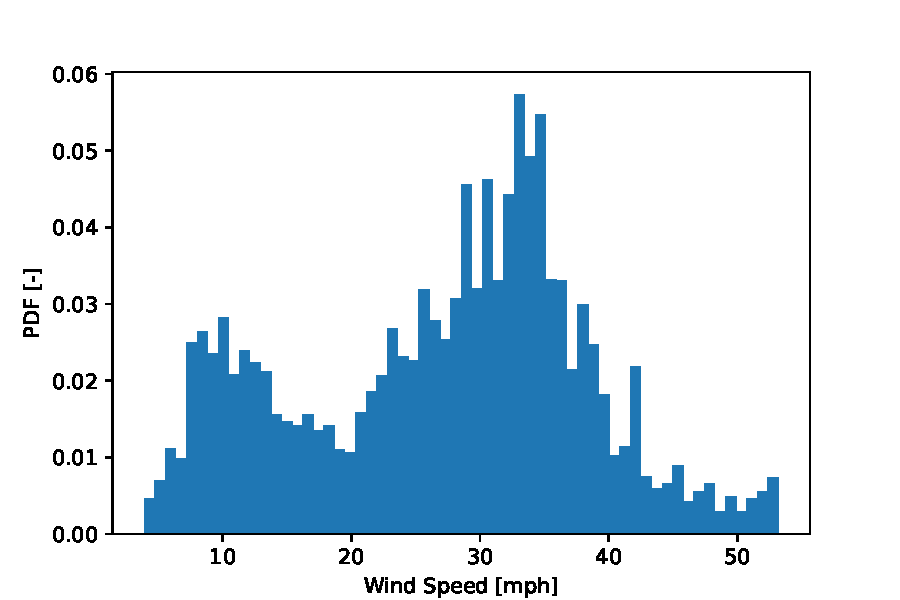
\includegraphics[width=0.7\textwidth]{../figures/hist_ws.pdf}
  \caption{Histogram of wind speed samples used in the ensemble.}
  \label{fig:hist_ws}
\end{figure}

\begin{figure}[h]
  \centering
  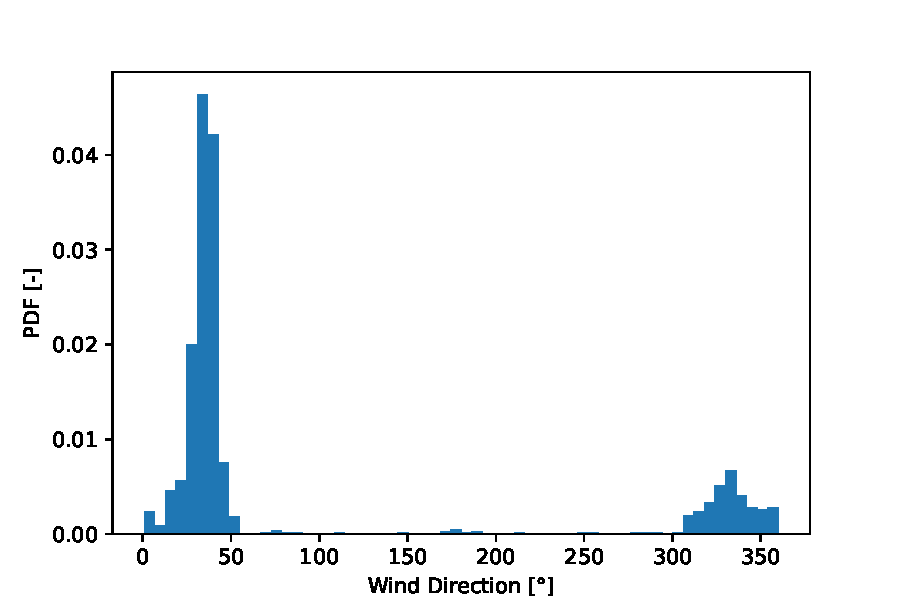
\includegraphics[width=0.7\textwidth]{../figures/hist_wd.pdf}
  \caption{Histogram of wind direction samples used in the ensemble.}
  \label{fig:hist_wd}
\end{figure}

\begin{figure}[h]
  \centering
  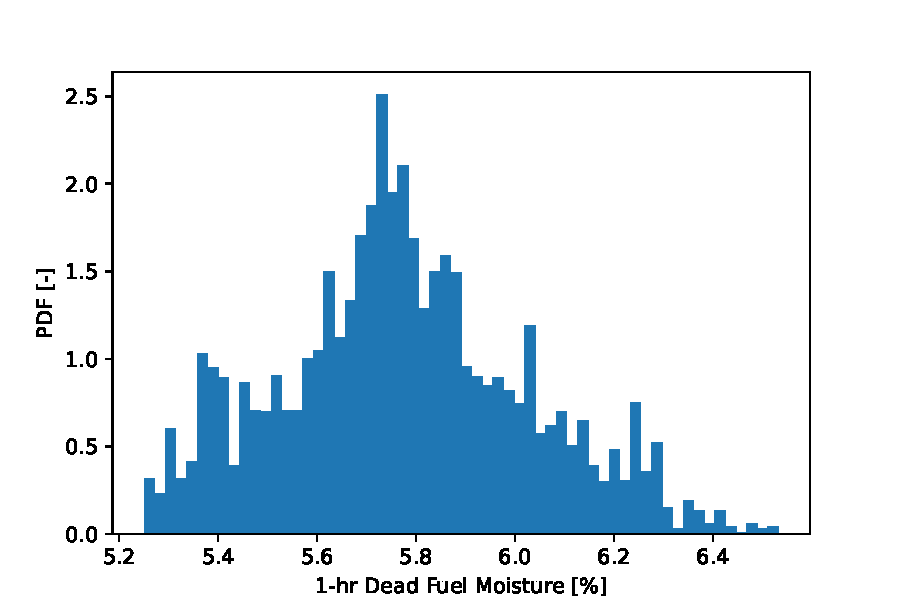
\includegraphics[width=0.7\textwidth]{../figures/hist_m1.pdf}
  \caption{Histogram of 1-hour fuel moisture content ($M_1$) samples.}
  \label{fig:hist_m1}
\end{figure}

\begin{figure}[h]
  \centering
  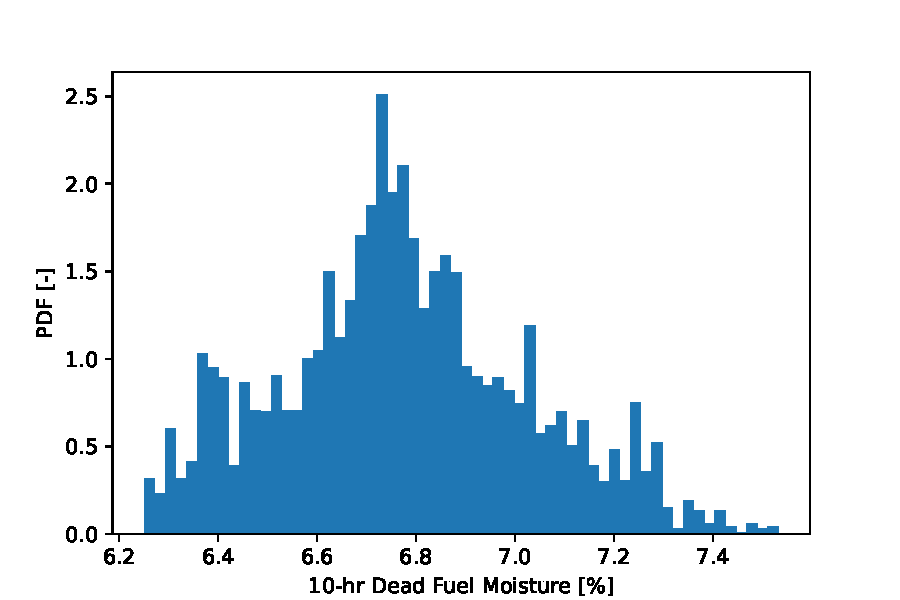
\includegraphics[width=0.7\textwidth]{../figures/hist_m10.pdf}
  \caption{Histogram of 10-hour fuel moisture content ($M_{10}$) samples.}
  \label{fig:hist_m10}
\end{figure}

\begin{figure}[h]
  \centering
  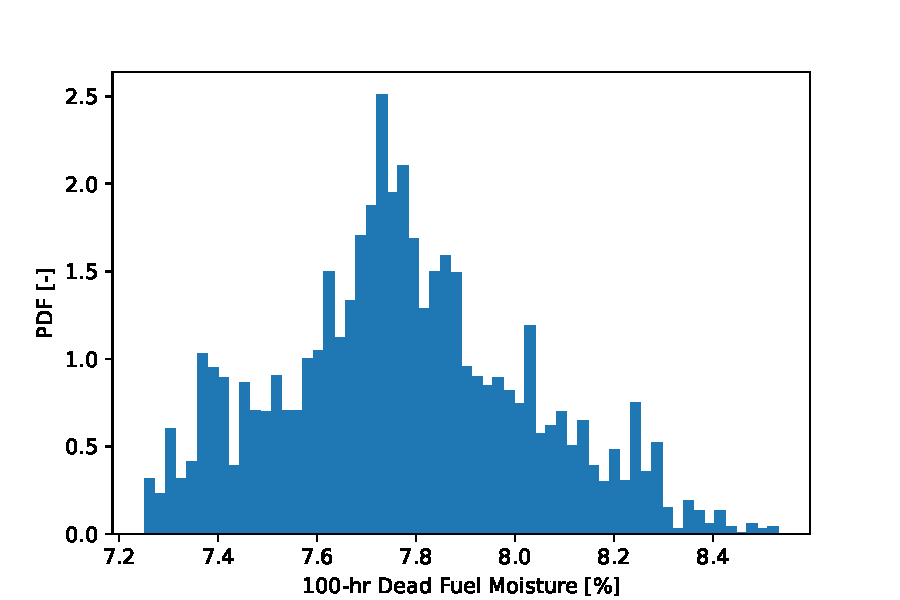
\includegraphics[width=0.7\textwidth]{../figures/hist_m100.pdf}
  \caption{Histogram of 100-hour fuel moisture content ($M_{100}$) samples.}
  \label{fig:hist_m100}
\end{figure}

\begin{figure}[h]
  \centering
  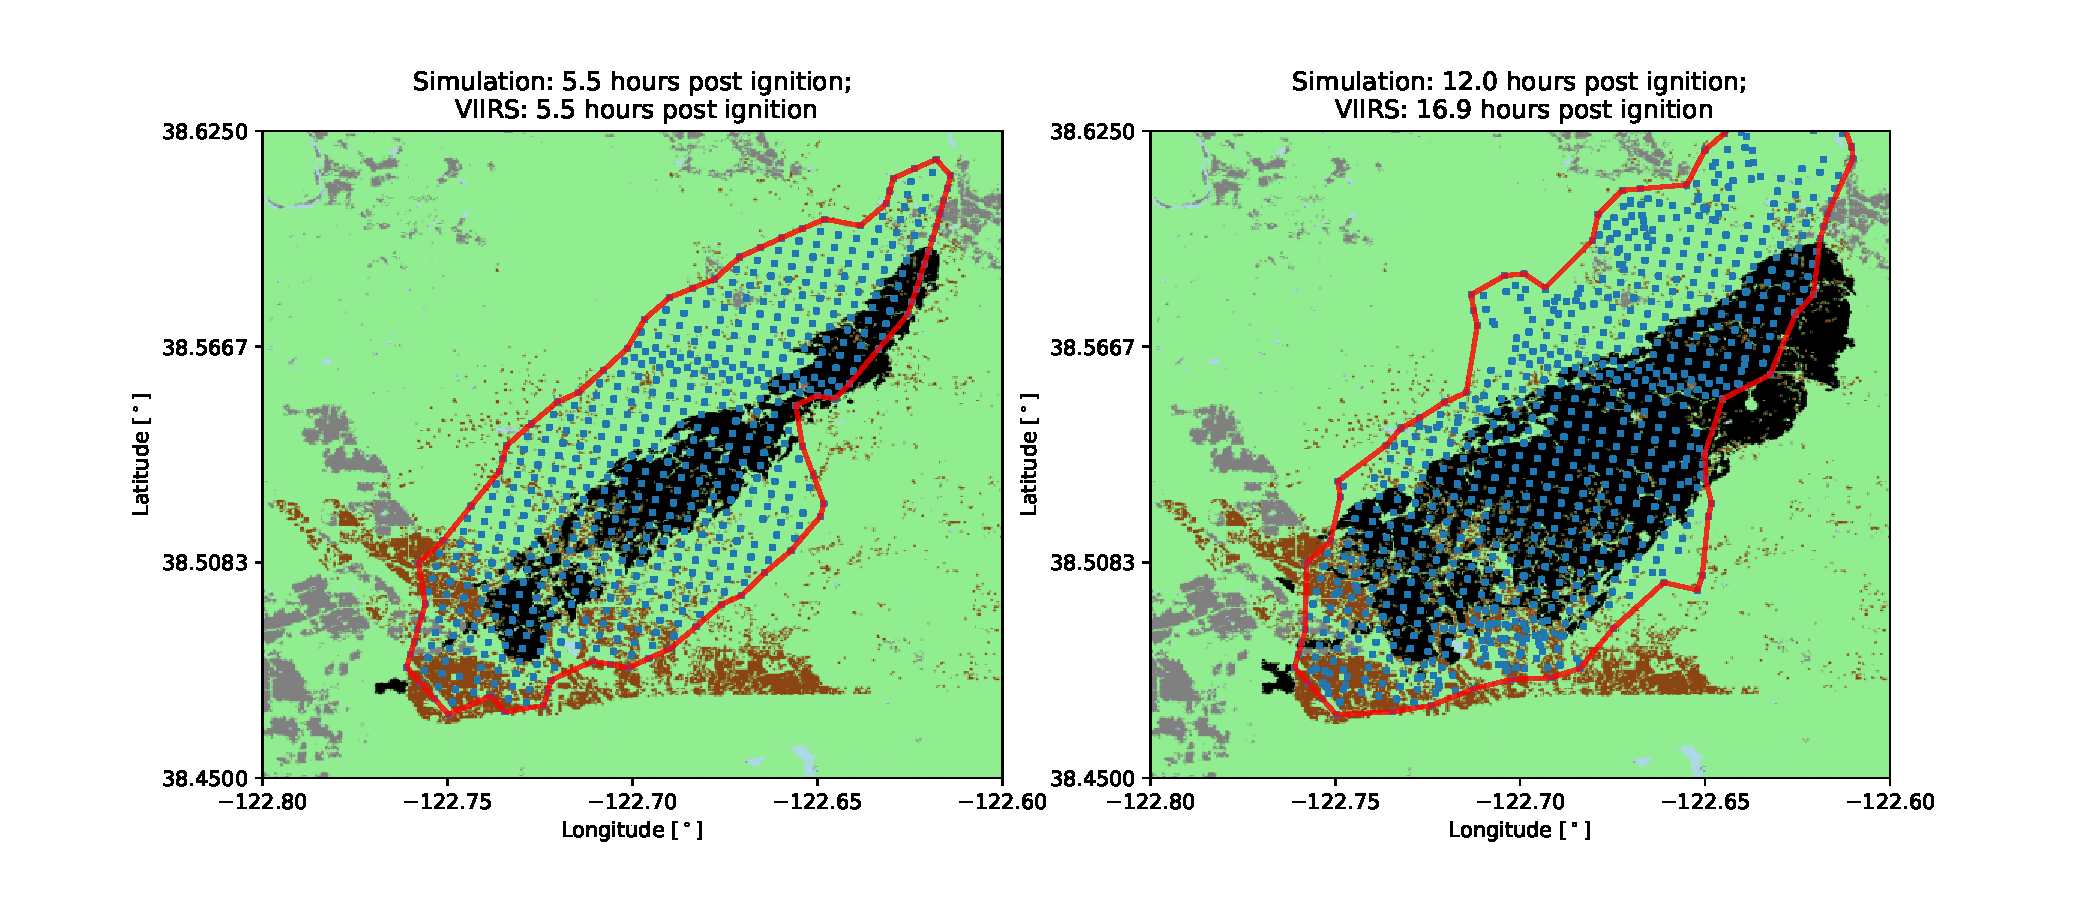
\includegraphics[width=1.0\textwidth]{../figures/simu_vs_viirs_examples.pdf}
  \caption{Examples of fire perimeter comparisons between simulations and VIIRS detections.}
  \label{fig:simu_vs_viirs_examples}
\end{figure}

\begin{figure}[h]
  \centering
  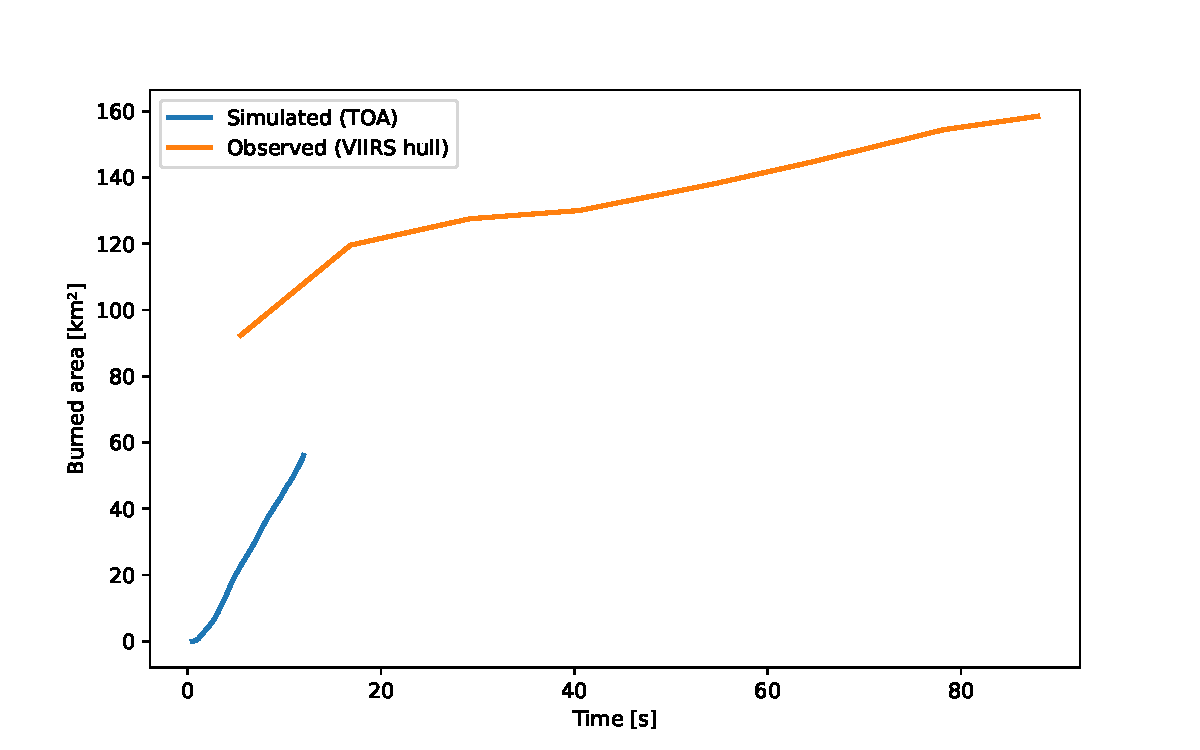
\includegraphics[width=0.7\textwidth]{../figures/burn_area_history.pdf}
  \caption{Time history of cumulative burned area from the ensemble simulations.}
  \label{fig:burn_area_history}
\end{figure}


\subsubsection{Key Metrics}
Summarize metric values (auto‑insert from JSON if desired in a later extension) and state Pass/Fail.


\subsection{Discussion}


\end{document}
